\section{Introduction}
Information retrieval is a widely employed technology that assists users in locating relevant information from extensive corpora, containing documents, web pages, and logging records \citep{bajaj2016ms,thakur2021beir}.
Relevant information can relate to user queries in different ways---sometimes through straightforward matching patterns like shared keywords or semantic similarities, and other times through deeper, more nuanced connections such as analogous underlying principles.
In many real-world scenarios, user queries can be highly complex, and finding the relevant documents requires intensive reasoning.
For instance, an economist might want to find a story explained by the same economic theory as another story, or a programmer might want to use an error message to locate the corresponding syntax documentation.
For these applications, relevant documents cannot be directly retrieved through lexical or semantic matching alone, but instead require additional reasoning steps to identify.

In this work, we study the problem of reasoning-intensive retrieval with \ours, a new benchmark that requires intensive reasoning to retrieve relevant documents.
Existing retrieval benchmarks, such as BEIR \citep{thakur2021beir} and MTEB \citep{muennighoff2022mteb}, primarily focus on fact-based queries typically derived from search engines, where the relevance between queries and documents is often straightforward and can be detected through simple keyword or semantic matching \citep{lee-etal-2019-latent,karpukhin2020dense}.
These datasets focus on retrieving specific pieces of information (e.g., ``the widest highway in North America''), which leads to the relevant documents often having high lexical or semantic overlap with the queries.
In contrast, the relevance between queries and documents in \ours is not easily detectable through simple keyword or semantic matching, and requires deliberate reasoning due to the complex nature of our domains and queries (\autoref{fig:main}).

\begin{figure}[t!]
  \centering
  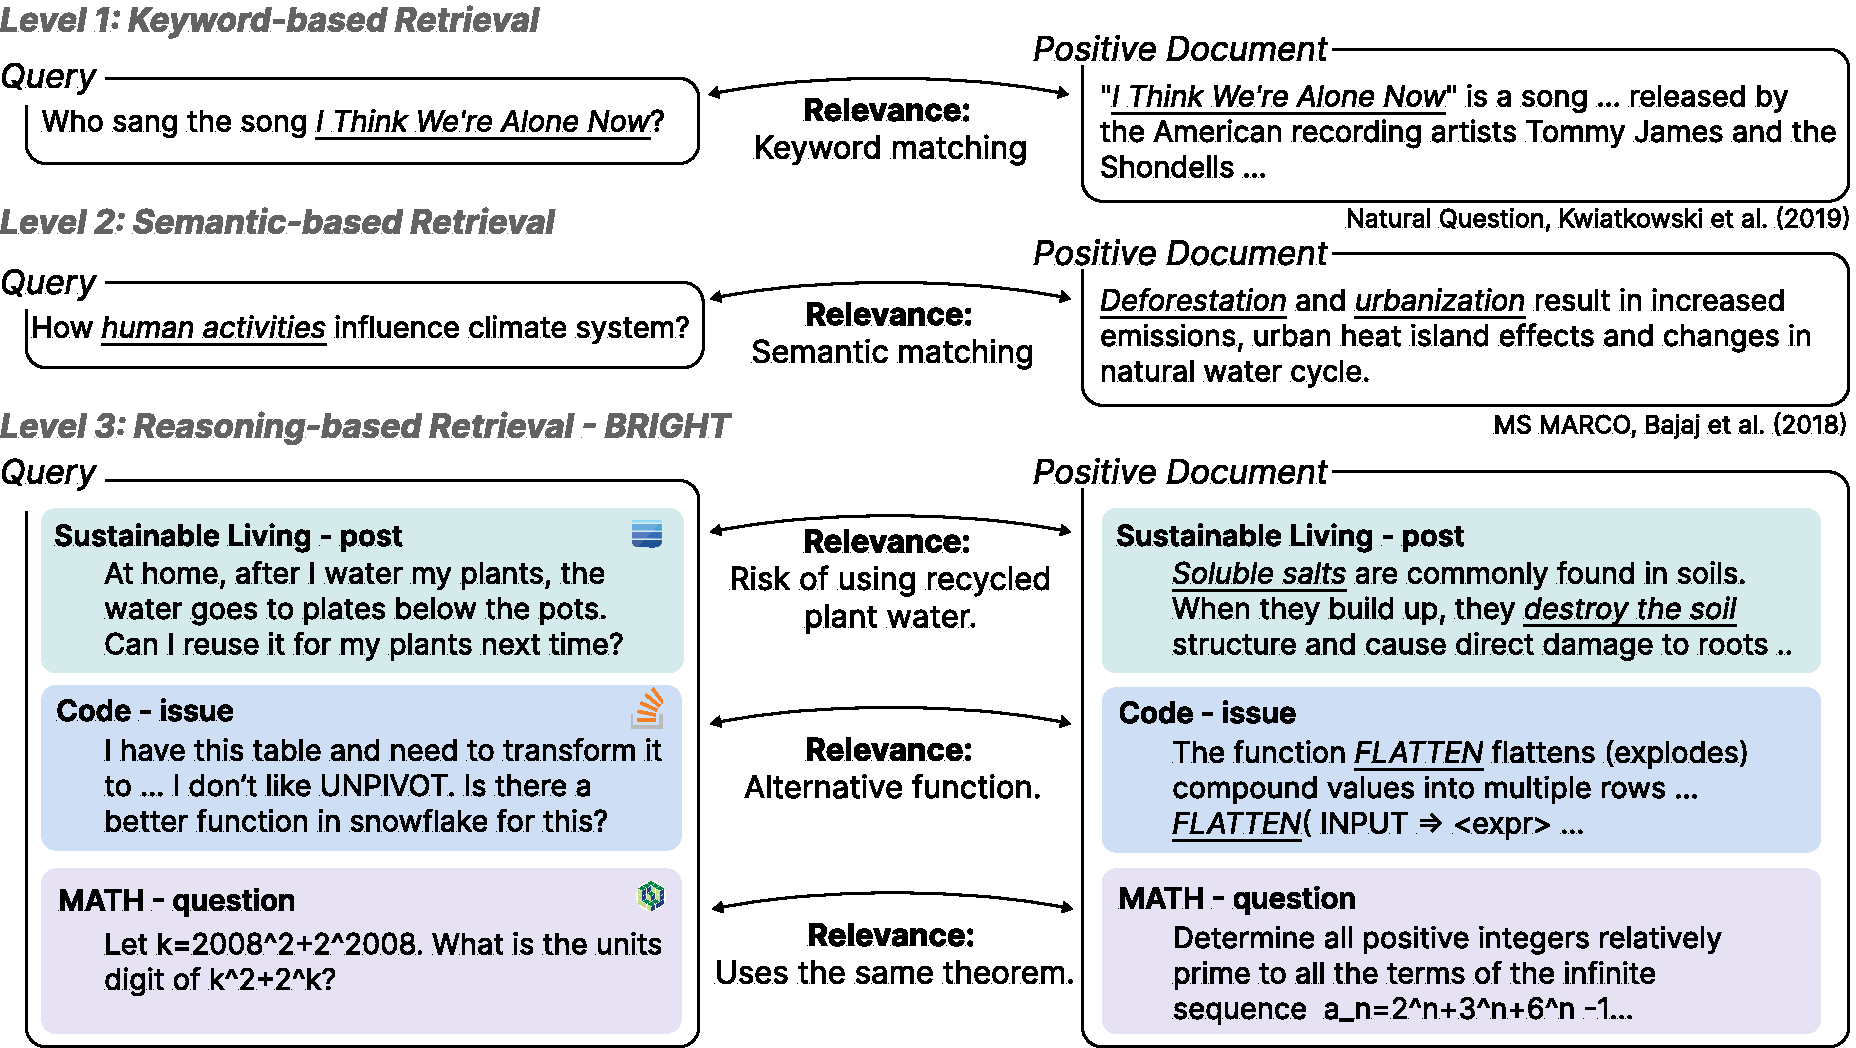
\includegraphics[width=\textwidth]{figures/figure1.pdf}
  \caption{Existing retrieval benchmarks focus on keyword-based retrieval (level 1), or semantic-based retrieval (level 2), e.g., NQ, MS MARCO datasets~\citep{kwiatkowski2019natural,bajaj2018ms}. 
  \textbf{\ours introduces level 3 retrieval, where the relevance between queries and documents requires intensive reasoning to determine.} 
  Our data consists of natural user queries from diverse domains (e.g., economics, math, earth sciences, etc.).
  % such as economics, psychology, robotics, software engineering, earth sciences etc.
  % In contrast to short questions with straightforward mapping to documents, \ours queries can contain long background descriptions without details on what to retrieve. \howard{i feel this sentence is duplicate of the first two sentences, as they express the same ideas.}
  % The paired documents might span blogs, syntax documentations, demonstration examples and more.
  \ours corpora also span across web data, such as blogs, syntax documentation, and STEM problem-solutions.
  }
  \label{fig:main}
\end{figure}

\ours consists of 12 datasets from diverse and advanced domains, sourced from naturally occurring human data and meticulously curated sources. The benchmark comprises two main components: 
1) seven datasets are constructed from StackExchange, where relevance is defined by whether a document is cited in the answer, and further validated through multiple annotators to ensure that the positive documents effectively support addressing queries. Given the inherent subjectivity of this assessment, we only include documents unanimously agreed upon by the annotators.
2) The remaining five datasets focus on coding and math problems, where the queries are inherently linked to the positive documents due to their shared underlying algorithms or theorems.

We evaluate 13 representative retrieval models of varying sizes and architectures. 
Comprehensive experiments highlight the challenges posed by \ours, as the best-performing model, SFR-Embedding-Mistral~\citep{meng2024sfrembedding}, which scores 59.0 on the MTEB retrieval subset, BEIR~\citep{thakur2021beir}, achieves only an nDCG@10 score of 18.3 on \ours.
To identify promising directions for improving \ours, we explore various strategies---one effective approach leverages LLMs to generate chain of thought reasoning steps~\citep{wei2022chain} about the query before retrieval, resulting in average improvements of up to 12.2 points. 
Furthermore, augmenting the downstream model with retrieved documents from the top-performing retriever, Qwen, enhances the question-answering performance compared to the closed-book setting.
However, using the oracle documents results in a larger improvement, highlighting the potential benefits of improving retriever models.

Moreover, our results demonstrate the robustness of \ours against potential data leakage during large-scale pre-training, as no substantial performance gains are observed even when models are further trained on documents from the benchmark dataset. 
We hope that our findings inspire research directions to advance the state of the art in reasoning-intensive retrieval.